
%%%%%%%%%%%%%%%%%%%%%%% xxxxxxxxxxxxxxxx %%%%%%%%%%%%%%%%%%%%%%%%%
%
%	copyright by Springer Heidelberg
%   http://www.springer.com/lncs       Springer Heidelberg 2006/05/04
%
%
%%%%%%%%%%%%%%%%%%%%%%%%%%%%%%%%%%%%%%%%%%%%%%%%%%%%%%%%%%%%%%%%%%%


\documentclass[runningheads,a4paper]{llncs}

\usepackage{amssymb}
\setcounter{tocdepth}{3}
\usepackage{graphicx}
\usepackage{caption}
\usepackage{url} %takes care of proper line breaks for URLs
\usepackage{hyperref} % creates clickable links and references.
\usepackage{float}% exact position of figures
\usepackage[backend=bibtex,natbib=true]{biblatex}
\bibliography{citations}

\setlength{\parindent}{0pt} % no indent on new paragraphs

\newtheorem{defn}{Definition}


\begin{document}

\mainmatter  % start of an individual contribution

% first the title is needed
\title{Domain Specific Modeling}

% a short form should be given in case it is too long for the running head
\titlerunning{Domain Specific Modeling}


\author{Tim Schneider\\ tim-1.schneider@uni-ulm.de}
\institute{Institute of Databases and
Information Systems, Ulm University}


\maketitle


\begin{abstract}
%The abstract should summarize the contents of the paper and should
%contain at least 70 and at most 150 words. It should be written using the
Nowadays computers and smartphones make it easier for both novices and domain experts to build 
and explore their own models and learn new scientific ideas in the process.
Domain Specific Modeling can support both experts and novices in building models for different domains.
There are approaches that enable novices with few or even no programming skills to implement their own models.
Domain experts on the other hand use modeling languages to create models to 
allow them to focus on domain-specific problems instead of implementation-specific details like supported 
language features of a programming language. 
In this paper we will give an brief overview over different domain-specific modeling langues with a focus on modeling languages for novices
as well as describe features offered by Xtext and GMF supporting the creation of textual and graphical modeling languages.
\end{abstract}

\section{Introduction}
\label{sec:introduction}
For centuries people from da Vinci to Einstein have created models [\ref{def:model}] to help them better 
understand patterns and processes in the world around them. 
Nowadays computers and smartphones have become an integral part of our everyday life, making
it easier to build our own models and learn new ideas in the process.
Domain Specific Modeling can support both experts and novices in building models for different domains.
There are approaches (e.g. LEGO Mindstorms,Starlogo) that enable novices with few or even no programming 
skills at all to implement their own models. Domain experts on the other hand use modeling languages 
(e.g. SimuLink,BPMN) designed for a specific domain to create models, which allows them to focus on 
domain-specific problems instead of implementation-specific details like supported 
language features of a general pupose programming language (e.g. C,C++,Java).
In this paper we will give a an overview about domain specific modeling languages for novices.
Additionally we will present the tools Xtext and GMF for creating textual and graphical modeling languages. 

% \begin{itemize}
%  \item can help experts and novices builing Models for different domains
%  \item enables novices with few or even no programming skills at all to implement their own models (e.g. MindStorm,Starlogo)
%  \item supports domain experts by setting focus on the domain-specific problems (e.g. SimuLink,BPMN)
%   \end{itemize}

\subsection{Foundation}
\label{subsec:introduction}
Before speaking about domain specific modeling languages we will give a short definitions for the  
terms \emph{model}(Def. \ref{def:model}),\emph{domain} (Def. \ref{def:domain}) and \emph{domain-specific modeling language}.

\subsubsection{Model}
% \begin{itemize}
%  \item What is a model? (Definition  [Stachowiak]
%  + some Explanation)
%  \item Abstraction: Remove details which do not serve the purpose
% 
%  \item Homomorphism: Statements on model elements hold for real world entities
%  \item Pragmatics: Model has some purpose
%  \item + example (novice) house Made of LEGOS $\rightarrow $ Model for a ``real'' house / building
%  \item + example (expert) blueprints from an architekt $\rightarrow $ different model, but  represents same object in real 
%  world
%  
%  \item Abstraction brings representational bias 
%  \item $\rightarrow$ electric cable installations, water pipes cannot be ``expressed'' in lego but they can with blueprints
%  \item $\rightarrow$ lego allows 3D Modeling while Blueprints cannot (oonly via 2d projections/ optical illusions)
%  \end{itemize}
%  
  \begin{defn}
    \label{def:model}
    A \underline{Model} is a formal representation of entities and relationships in the real world (abstraction) 
    with a certain correspondence (homomorphism) for a certain purpose (pragmatics) \cite{stachowiak1973allgemeine}.
  \end{defn}
  
  This definition contains three aspects: abstraction, homomorphism, pragmatics.
  A model should create a simplified view on the represented entities and relationships and 
  only contain details which are relevant (abstraction).
  Additionally statements on the model elements should hold for the represented entities and relationships (homomorphism).
  The question which details are relevant and should be included in the model is determined by the purpose of a model (pragmatics).  
 
  Creating models is something we do in our everday lifes:
  When building a house in LEGO a child creates a model which serves as a representation for a building in the real world.
  It is a simplified view on the original as it abstracts from detais like used materials, installed cables and water pipes and focusses
  on the shapes of the building.
  Another example for creating models is an architekt, who creates blueprints for some house, serving as a model for it.
  Blueprints contain 2D projections of walls and installations in that house from different viewpoints and abstract from the original by ommiting
  details like materials and some 3D information. 
  We can see from this example that these abstraction also brings a representational bias:
  Electric cable installations and water pipes cannot be modeled in LEGO but they can with blueprints.
  LEGO models on the other hand allows to model structures directly in 3D while blueprints cannot.
  
  Although novices (e.g. the child) and experts(e.g. the architect) may have different views on the same thing (e.g. the house)
  they share a common understanding in the concepts of the real world.  
  \begin{defn}
    \label{def:domain}
    A \underline{Domain} is the common knowledge of the requirements, concepts and functionality in a field of study.
  \end{defn}
  Despite their different level of expertise, both experts and novices know that the concepts ``wall'' and ``roof'' are 
  related to parts of a building and that a house needs both to be a valid house.
%  \begin{itemize}
%  \item novice and expert have different views on the same thing  but use different models / languages
%  \item both models may be used in the context of a domain (Architekture)
%  \item What is a Domain? (Definition + some Explanation)
%  \end{itemize}
  \begin{defn}
    \label{def:domainspecificmodelinglanguage}
    A \underline{Domain Specific Modeling Language} is a textual or graphical representation 
    of the concepts, entities and relationships that are relevant for a specific domain.
  \end{defn}
 \subsection{Domain-Specific Modeling Languages}
 The pupose of a domain-specific modeling languages is to support users in building models for a specific domain.
 Definition \ref{def:domainspecificmodelinglanguage} implies that there are two different kinds of modeling languages:
  \begin{description}
     \item[Graphical Modeling Languages] use graphical shapes, lines and arrows  to represent entities and relationships from the real world.
     \item[Textual Modeling Languages] use textual descriptions to represent entities and relationships from the real world.
  \end{description}
 The same model may be expressed in both, a graphical or textual modeling languages.
 For example: A finite state machine can be represented as a set of nodes, labeled boxes and arrows, while it can also be 
 represented by a textual description following a grammar to represent the same finite state machine.
  \begin{figure}[H]
      \centering
      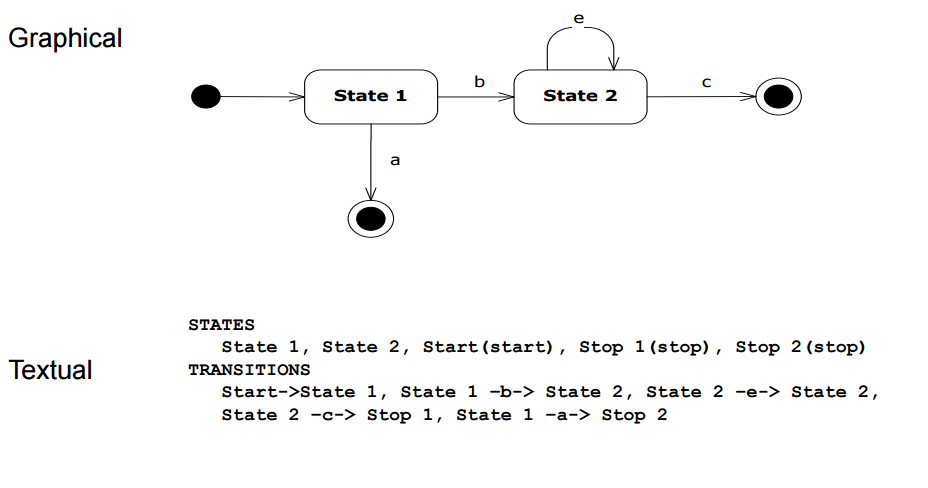
\includegraphics[width=\textwidth]{images/GraficalTextualComparison.PNG}
      \captionof{figure}{Comparison between textual modeling language and graphcal modeling language for the same model of a finite state machine.}
      \label{compare:textgraphiclang}for the
    \end{figure}
 The decision whether a graphical modeling language or textual modeling language is chosen for the implementation of a modeling tool 
 may also be influenced by the targeted audience: A software-developer has a deep knowledge in using text-based editors, while 
 children may not have these kind of expertise and therefore prefer a more graphical representation. 
 Different levels of expertise can also be observed with regards to domain knowledge:
 A software-engineer probably has a more detailed knowledge in the computer science domain compared to a medical doctor.
 We will therefore distinguish between domain experts and novices. 
 Additionally, we will focus on domain-specific languages for novices in this paper.
 %  \begin{itemize}
%  \item different approaches :  Graphical Modeling Languages, Textual Modeling Languages
%  \item 
%    \begin{figure}[ht]
%       \centering
%       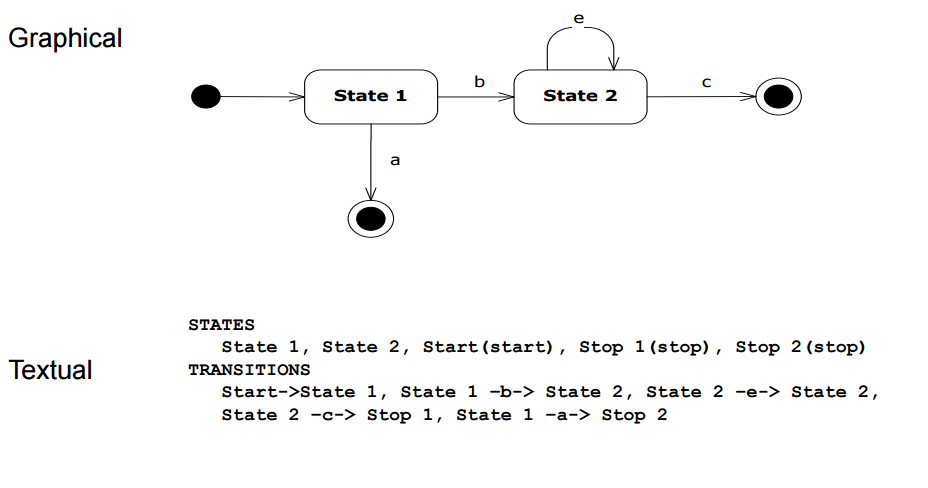
\includegraphics[width=\textwidth]{images/GraficalTextualComparison.PNG}
%       \captionof{figure}{comparison between textual modeling language and graphcal modeling language for the same model}
%     \end{figure}
%  
%  \item examples (domain experts): BPMN , SimuLink
%  \item examples (novice ): STARLOGO 
%  \end{itemize}
 
 \section{Domain-Specific Modeling Languages for Novices}
 As there is a variety of software tools available, which implement different modeling languages, this section will give an overview 
 about modeling languages designed to support novices with few or even no programming languages in creating models and help them better 
 understand patterns and processes in the world around them.
 
 \subsection{StarLogo TNG}
  %enable students to build simulations and learn features of complex systems without extensive background knowledge (Klopfer et al., 2009a; 2009b)
  %provides an environment for building agent-based models
  StarLogo is a client based modeling software, developed specifically to enable students to 
  create models for the simulation of complex systems without extensive programming skills \cite{klopfer2009starlogo}.
  It provides a graphical modeling language using blocks instead of a textual syntax. 
  These blocks are coloured based on the function they have in the program and their shapes only allow syntactically correct constructs \cite{klopfer2009starlogo}.
  This eases the learning of basic programming concepts such as control-flow (e.g. loops, if-then statements),
  assignments and methods by providing intuitive graphical mappings. Since StarLogo TNG uses these puzzle-piece shapes, understanding 
  control-flow, for example, ``requires little more than visually parsing the if or repeat commands 
  to conclude that items placed within the then slot will be performed if the items placed within the 
  test slot are true, or the items placed within the do slot will be subject to the number of repetitions placed within the times slot''\cite{smith2011biology}.
  Using puzzle-piece shapes for basic programming concept avoids syntactic errors, 
  which are one of the main difficulties in learning textual programming languages.
  Figure \ref{fig1} shows an exmaple for the blocks used by StarLogo TNG: 
  the curved shape of a Boolean variable is easy to distinguish from the pointed shape of a number value.
  
  \begin{figure}[H]
	\centering
  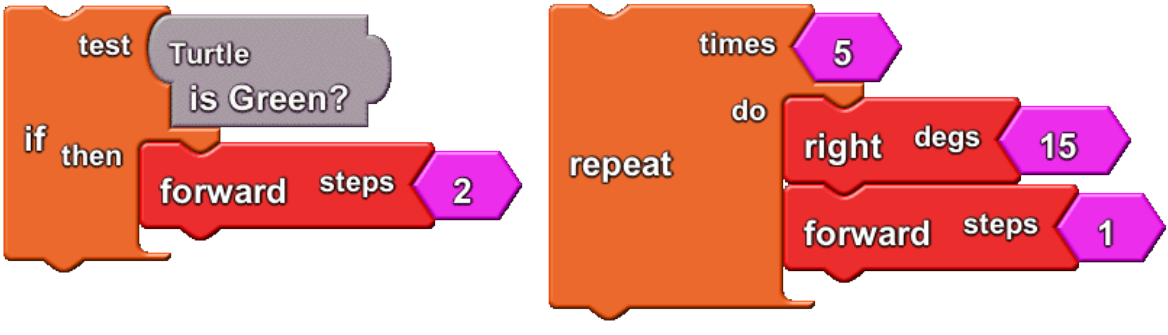
\includegraphics[width=0.5\textwidth]{images/StarLogoTNGBlocksEx.PNG}
	\caption{ StarLogo TNG’s graphical programming blocks. Example if (left) and repeat (right) blocks are shown. The
	  if block commands a Turtle agent to take two steps forward if it is green; the repeat block commands an agent to
	  repeat five times the sequence of turning right 15 degrees and taking one step forward. (from \cite{smith2011biology})}
	\label{fig1}
  \end{figure}
  
  %   \begin{itemize}
%   \item is a client-based modeling and simulation software
%   \item enables secondary school students and teachers to model decentralized systems through agent-based programming
%   \item facilitates the creation and understanding of simulations of complex systems
%   \item graphical programming blocks instead of text-based computer code
%   \end{itemize}

   \subsection{Scratch}
  Scratch is graphical modeling languages for visual programming that allows users (primarily ages 8 to 16\cite{maloney2010scratch}) to learn
  computer programming while working on personally meaningful projects such as animated stories and games. 
  A major design goal of Scratch is to support self-directed learning through tinkering and collaboration with peers \cite{maloney2010scratch}. 
  Scratch uses blocks \ref{scratchblocks} similiar to StarLogoTNG for creating models. One of the key features of Scratch is that it is always \emph{live},
  which means that there is no compilation step or edit/run mode distinction. A user can see what a command or program fragment does by clicking 
  it at any time. This also implies that a user can change parameters or add new blocks to a script while it is running.
  Because it is live Scratch encourages users to experiment with it and supports
  a bottom-up approach to writing scripts where small chunks of program fragments are assembled and tested, then combined into larger units.
  Additionally Scratch provides visual feedback to show script execution by surrounding a script with a white border when it is 
  running (Fig. \ref{scratchlive}). This feedback
  helps the user understand when scripts are triggered and how long they run. If an error is encountered then border of the 
  affected script turns red and the block that caused the error is highlighted in red. 
  Furthermore Scrach eliminates the need syntax error messages by using 
  puzzle-piece shapes which only fit where it makes sense. Additionally Scratch tries to avoid runtime errors by making all blocks be
  \textit{failsoft}. ``Rather than failing with an error message, every block attempts to do something sensible even when presented with out-of-range inputs''\cite{maloney2010scratch}.
  Even though eliminating the runtime error messages does not eliminate the errors,by following this apprach a script can always be tested by the user.
  Since a program that can be tested even if the result is incorrect it is favoured to not be able to run or compile it at all.

     \begin{figure}[H]
      \centering
      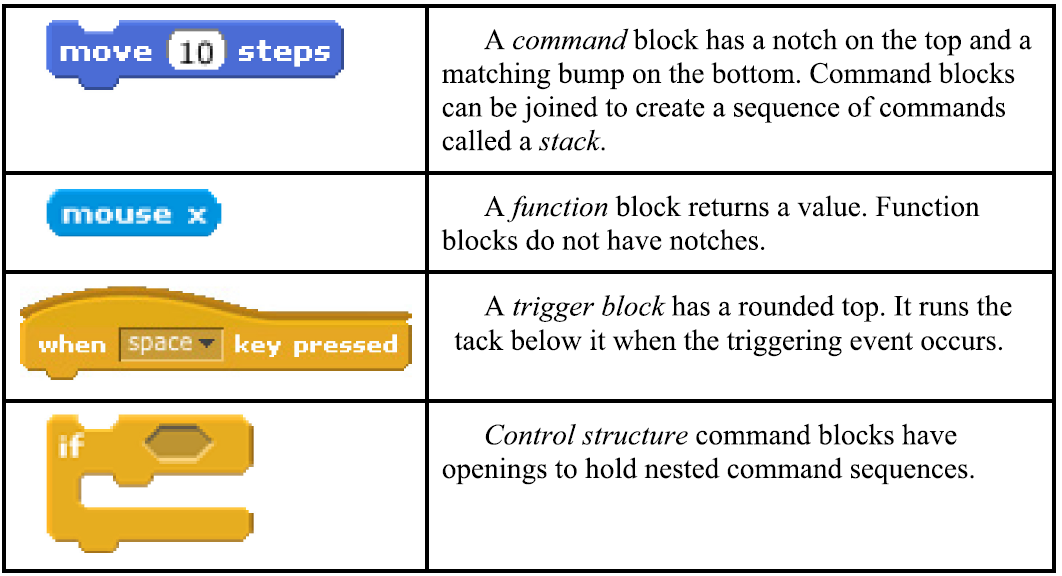
\includegraphics[width=.7\textwidth]{images/ScratchBlockTypes.PNG}
      \captionof{figure}{Scratch Block Types(from \cite{maloney2010scratch})}
       \label{scratchblocks}
    \end{figure} 
        \begin{figure}[H]
      \centering
      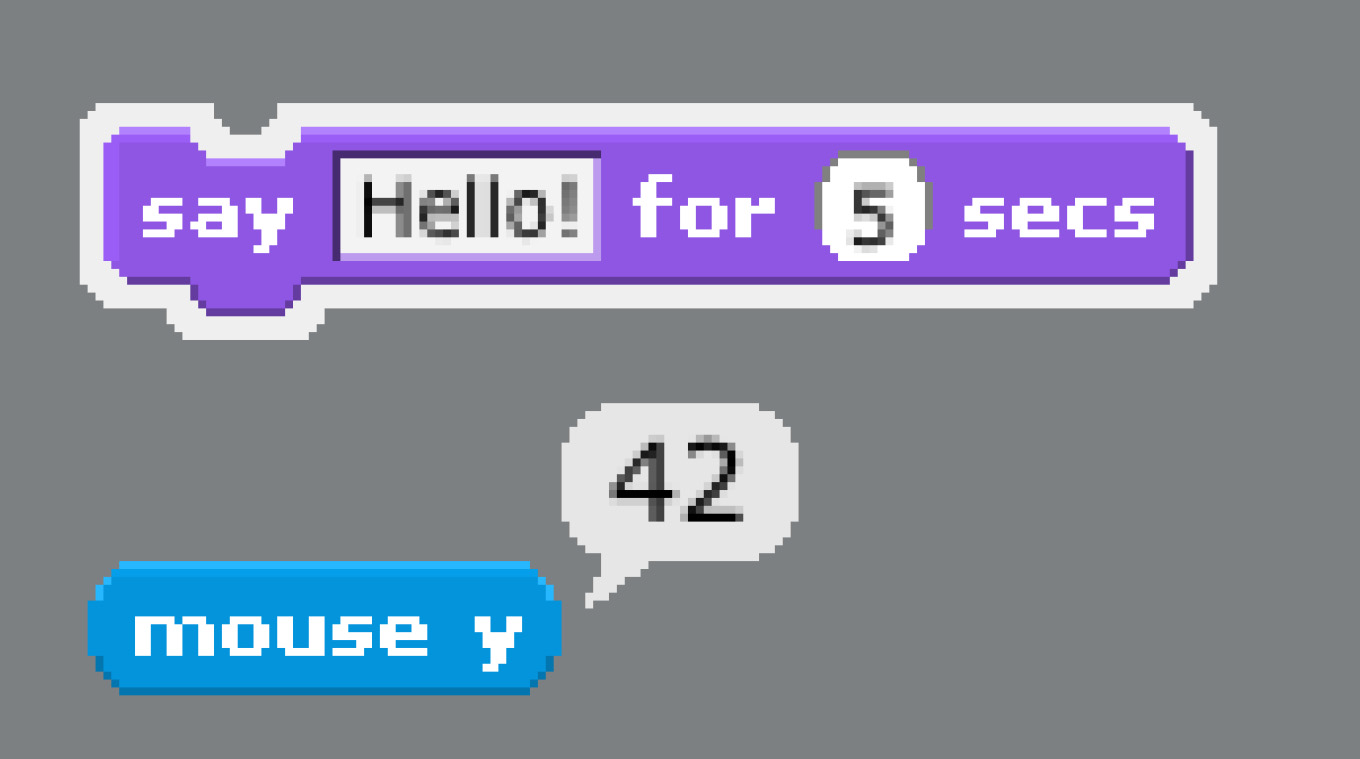
\includegraphics[width=.7\textwidth]{images/ScratchLive.png}
      \captionof{figure}{Blocks can be tested simply by clicking on them. A white border indicates that a block or
      stack is running. Function blocks show their output in a  bubble.(from \cite{maloney2010scratch})}
      \label{scratchlive}
    \end{figure}
    \begin{figure}[H]
      \centering
      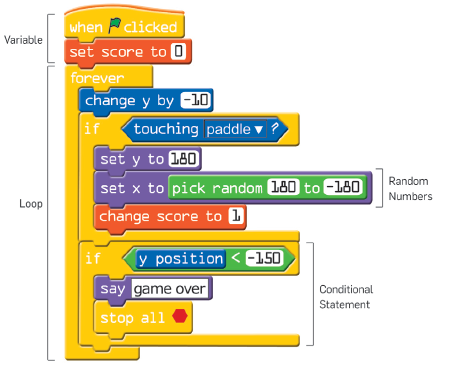
\includegraphics[width=.7\textwidth]{images/Snatch1.PNG}
      \captionof{figure}{Sample Scratch script (from Pong-like paddle game) highlighting computational and mathematical concepts}
    \end{figure} 
   
  \newpage
  \subsection{PhyDSL}
  Both StarLogo and Scratch use graphical modeling languages for creating models. 
  \emph{PhyDSL} is a tool, designed as an Eclipse\cite{eclipse} plugin that uses a textual modeling language for creating models for the game development domain.
  It was designed for the purpose of supporting the fast prototyping of physics-based games, including platform, shoot ’em up, 
  puzzle and maze games \cite{guana2014phydsl}. 
  The provided frontend includes a text editor (including syntax highlighting and text completion), which is used to define gameplay in highlevel
  terms describing the gameplay static, dynamic elements and their behaviors by a domain-specific modeling language.  
  It is based on the \emph{Eclipse Modeling Framework}\cite{gronback2009eclipse} (EMF) and uses codegeneration for deriving C\# code supported by Microsoft’s
  DirectX API. 
  The modeling language provided by PhyDSL consists of four gameplay definition sections: mobile and
  static actor definition (Fig. \ref{actordef}), 
  environment and layout definition (Fig. \ref{envdef}), 
  activities definition (Fig. \ref{activitiesdef}), 
  and scoring rules definition (Fig. \ref{rulesdef}).
  
%  \begin{itemize}
%   \item textual modeling for (simple) game dev domain
%   \item based on EMF
%   \item allows codegeneration from the created models
%   \item mobile gameplay definition sections:
%     \begin{itemize}
%     \item static actor definition
%     \item environment and layout definition
%     \item activities definition
%     \item scoring rules definition
%     \end{itemize}
%   
%   \end{itemize}
     \begin{figure}[H]
      \centering
      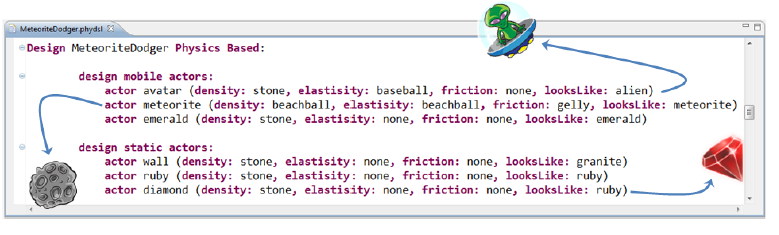
\includegraphics[width=\textwidth]{images/PhyDSL1.PNG}
      \captionof{figure}{PhyDSL: Static Actor Definition (from  \cite{guana2014phydsl})}
      \label{actordef}
    \end{figure}
      \begin{figure}[H]
      \centering
      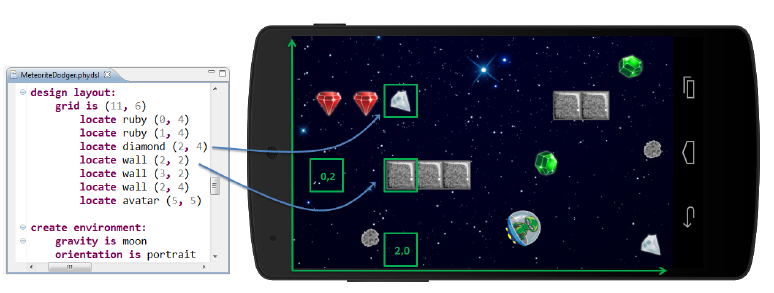
\includegraphics[width=\textwidth]{images/PhyDSL2.PNG}
      \captionof{figure}{PhyDSL: Environment and Layout Definition(from  \cite{guana2014phydsl})}
      \label{envdef}
    \end{figure}
  \begin{figure}[H]
      \centering
      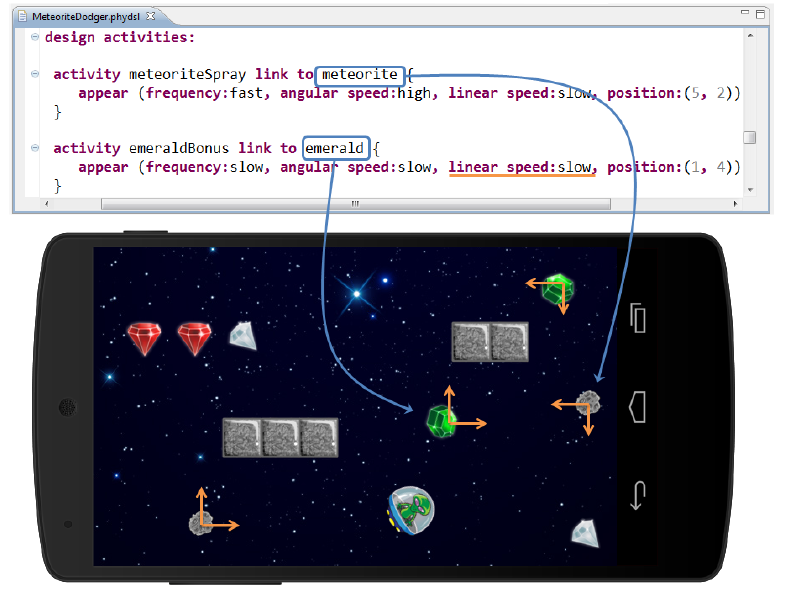
\includegraphics[width=\textwidth]{images/PhyDSL3.PNG}
      \captionof{figure}{PhyDSL: Activities Definition(from  \cite{guana2014phydsl})}
      \label{activitiesdef}
    \end{figure}

\begin{figure}[H]
      \centering
      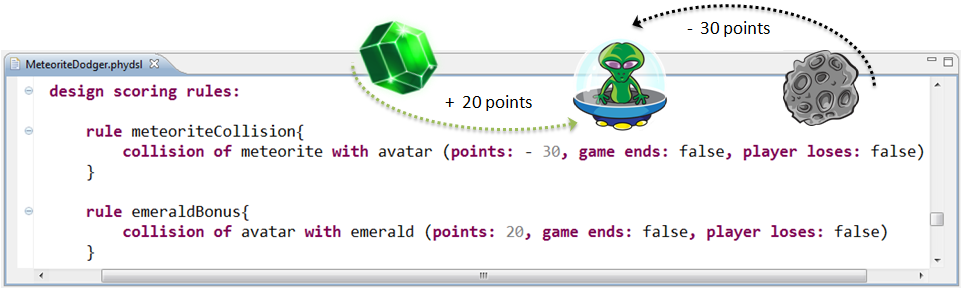
\includegraphics[width=\textwidth]{images/PhyDSL4.PNG}
      \captionof{figure}{PhyDSL - Scoring Rule Definition for Collision Rules (from  \cite{guana2014phydsl})}
      \label{rulesdef}
    \end{figure}

   \pagebreak
   
   \subsection{LEGO Mindstorms}
   Another example for a graphical modeling language made for novices is the EV3 Programmer App \ref{fig:ev3app}
   for LEGO Mindstorms which includes a block-based graphical modeling langue for creating programms
   for the LEGO MindStorm Robots. Programs are loaded and executed on a EV3 Programmable Brick (Fig. \ref{ev3pbrick}), 
   which offers input and output connections for interaction with sensors and actuators.
   Different colors are used to indicate whether a blocks triggers some action (green; Fig. \ref{fig:actionblocks}), is used for flow control (orange; Fig. \ref{fig:flowblocks}),
   reads data from some input (e.g. color sensor)(yellow; Fig.\ref{fig:sensorblocks}) or trigger some data operation (e.g. read/write some variable) (red; Fig. \ref{fig:operationsblocks}).
   
%   \begin{itemize}
%   \item EV3 Programmer App or Computer Software for programming lego robots in a graphical syntax 
%   \item action blocks (green), flow blocks (orange), sensor blocks (yellow), data operation blocks (red), advanced blocks (dark blue)
%   \item programms are executed on the EV3 P-brick. 
%   %https://www.lego.com/en-us/mindstorms/learn-to-program
%   \end{itemize}
  
  \begin{minipage}{.5\textwidth} %
	  \centering
    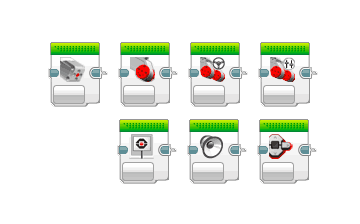
\includegraphics[width=\textwidth]{images/LearnToProgram_action_blocks_landscape.png}
	  \captionof{figure}{The action blocks control the actions of the program, e.g. motor rotations, image, sound and the light on the EV3 P-brick (from \cite{legoev3}).}
	  \label{fig:actionblocks}
  \end{minipage} %
  \begin{minipage}{.5\textwidth} %
	  \centering
    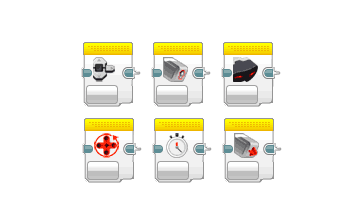
\includegraphics[width=\textwidth]{images/LearnToProgram_sensor_blocks_landscape.png}
	 \captionof{figure}{The sensor blocks allow to read the inputs e.g. from a color sensor, IR sensor, touch sensor (from \cite{legoev3}).}
	 \label{fig:sensorblocks}
  \end{minipage}
  \begin{minipage}{.5\textwidth} %
	  \centering
    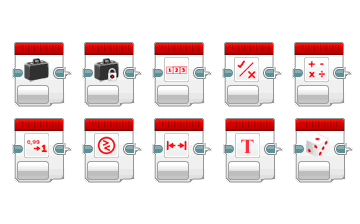
\includegraphics[width=\textwidth]{images/LearnToProgram_operations_blocks_landscape.png}
    \captionof{figure}{The data operation blocks let the user write and read variables, compare values for example (from \cite{legoev3}).}
    \label{fig:operationsblocks}
  \end{minipage}
  \begin{minipage}{.5\textwidth} %
	  \centering
    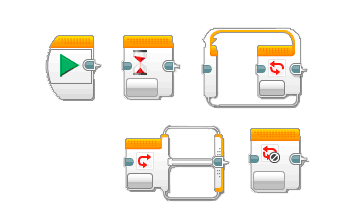
\includegraphics[width=\textwidth]{images/LearnToProgram_flow_blocks_landscape.png}
    \captionof{figure}{The Flow blocks control the flow of the program (from \cite{legoev3}).}
    \label{fig:flowblocks}
  \end{minipage}
  
    \begin{figure}[H]
	  \centering
    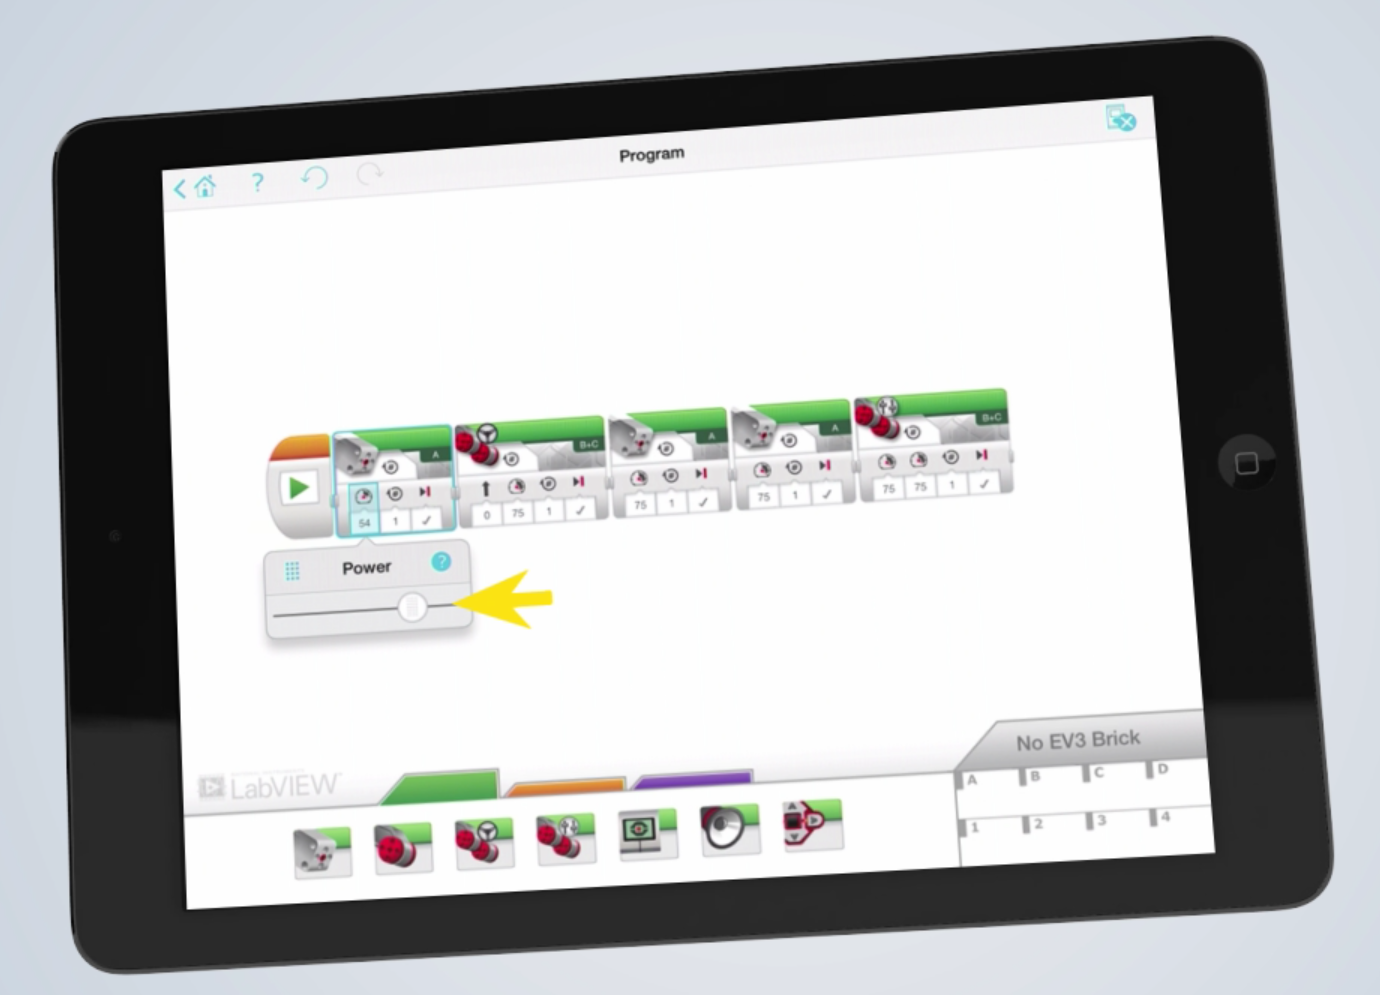
\includegraphics[width=0.5\textwidth]{images/mindstorms0.PNG}
	  \caption{EV3 Programmer App on a tablet used to create programms using a graphical modeling language (from \cite{legoev3}).}
	  \label{fig:ev3app}
    \end{figure}


      \begin{figure}[H]
	        \centering
      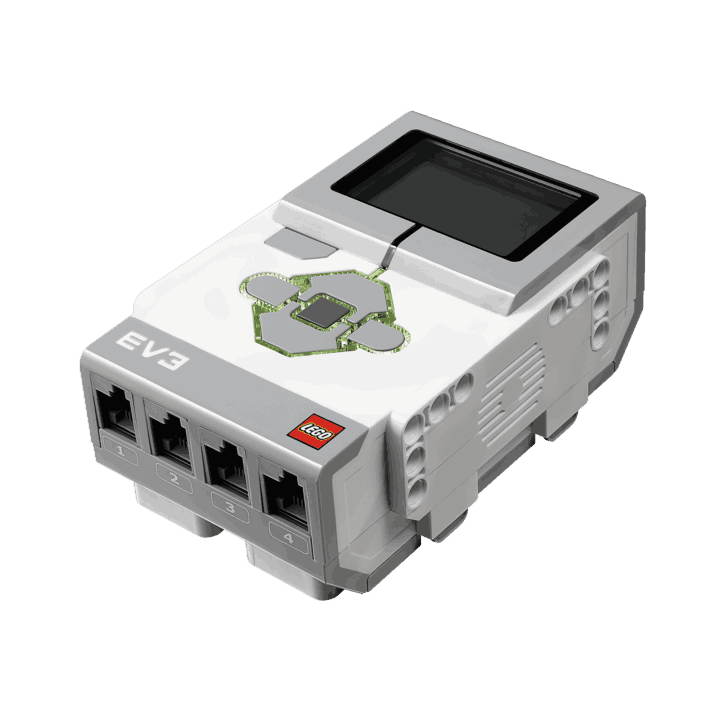
\includegraphics[width=0.5\textwidth]{images/ev3brick.png}
	    \captionof{figure}{EV3 Programmable Brick with connections for different sensors and actuators (from \cite{legopbrick}).}
	    \label{fig:ev3pbrick}
      \end{figure}


%     \subsection{Sensr}
%     \begin{itemize}
%      \item enables people without programming skills to build mobile data collection and management tools for citizen science
%     \end{itemize}

    
    \newpage
    \section{Creating Domain-Specific Modeling Languages}
    Domain-Specific Modeling Languages are implemented in various software tools using textual or graphical modeling languages.
    In fact, there are approaches to define these modeling languages as models using some kind of meta-language.
    Xtext and GMF are implementions for the Eclipse Modeling Framework (EMF), which adopt this approach.
    
    \subsection{Xtext}
    Xtext is a framework for development of programming languages and domain-specific modeling languages \cite{eysholdt2010xtext}.
    It uses a syntax similar to extended backus-naur form (EBNF) to describe custom textual modeling languages. 
    From this modeling language definition Xtext generates a custom Text-Editor for Eclipse whose features include code-completion and syntax-highlighting
    as well as a parser for parsing models from text files specified in the defined grammar. This makes it easy for experts of the language design
    domain to create models for custom modeling languages without programming skills or knowledge on how to implement a parser.
    As the modeling language definitions are stored in the Ecore format \footnote{Ecore is a (meta-)model included in the Eclipse Modeling Framework (EMF), which is used to describe with elements, attributes and relationships are allowed 
    in a model. It is an implementation of the \emph{Meta Object Facility} (MOF) Standard \cite{mof20062}, specified by the OMG.}, other tools in the EMF framework can process data from the parsed 
    models (e.g. Acceleo\cite{musset2006acceleo} for performing codegeneration).  
    
    \begin{figure}[H]
      \centering
      \label{fig:fsmgrammar}
      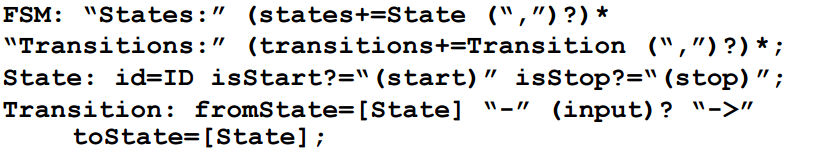
\includegraphics[width=\textwidth]{images/XTextGrammar.PNG}
      \captionof{figure}{Xtext grammar of a textual modeling language for finite state machines. 
      Figure \ref{compare:textgraphiclang} contains an textual description of a state machine 
      which follows this grammar definition.}
    \end{figure}
   
%     \begin{itemize}
%       \item used to create textual DSLs for ecore (meta-)models designed in EMF
%       \item syntax similar to EBNF
%       \item one rule for each (meta-)model element
%     \end{itemize}
%    
    
    \subsection{GMF}
    The Eclipse Graphical Modeling Framework(GMF \cite{gmf}) provides a generative component and runtime infrastructure for developing 
    editors for graphical modeling languages for models created in the Eclipse Modeling Framework.
    For creating a graphical modeling language a domain model must be given in the Ecore format.
    GMF uses a mapping model for the generation of a eclipse plugin for a custom graphical modeling language for the provided domain model. 
    Each element of the domain model is mapped to an element of a graph model, containing user defined shapes and arcs as representations for elements 
    and relationships of the domain model. Fig \ref{mapmodel} shows which models are used for the creation of a custom graphical modeling language.
    This example uses the finite states machine domain model, which must be predefined using Ecore. 
    The Ecore model contains elements like ``Finite State Machine'', ``Transition'' , ``State'',``StartState'', ``EndState'', ... .
    Additionally a graph model must be created, which contains all the shapes that we want to 
    use as a representation for some element from the domain model. This includes circles for Start- and EndState , Boxes for States,
    and arrows for transitions. To actually assign a shape to some domain model element a reference between model element from the domain model 
    and some shape of the graph model must be added to the mapping model. Finally one has to define which elements can be created using the context 
    menu in the generated graphical editor.

    \begin{figure}[ht]
      \centering
      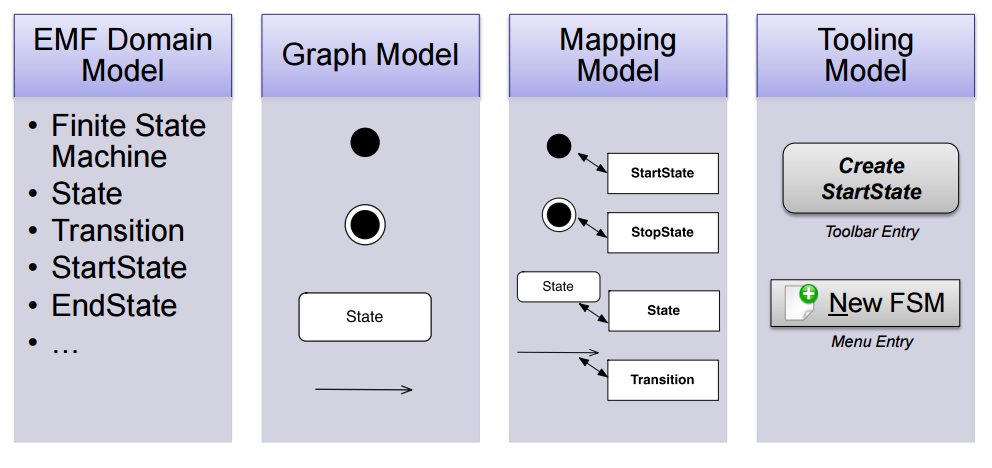
\includegraphics[width=\textwidth]{images/TableGMFSteps.PNG}
      \captionof{figure}{Models needed to create a graphical editor using GMF.}
      \label{mapmodel}
    \end{figure}
    
\section{Summary}\label{sec:summary}
Domain-specific modeling languages allow novices to build and explore  their own models and learn new scientific ideas in the process.
An overview over different domain specific modeling languages and the features they provide for 
supporting novices in the process of creating valid models is provided.
The modeling languages were selected due to their focus on supporting novices with few or even no programming skills.

Additionally it is presented how domain specific modeling languages can be created using some kind of meta-languages
for describing both custom textual and graphical modeling languages using Xtext and GMF as an example.

The presented tools for creating custom textual and graphical modeling languages could be used in for the simple creation of new intuitive and 
novice orientated modeling languages for other domains. PhyDSL is some exmaple, how Xtext can be used to create textual domain-specific modeling languages 
for novices was and future research project may use Xtext and GMF or similiar tools for fast developent of specialised domain-specific modeling languages.  

% 
% ---- Bibliography ----
% 
%\nocite{*}

%\bibliographystyle{splncs}
%\bibliography{citations}
\printbibliography
\end{document}

